\chapter{Results and Discussion}
The main focus during this project rested on two distinct qubit designs, namely the interdigitated and the parallel pad qubits. The two designs can be compared in figure \ref{fig:}. First, the influence of different parameters on the capacitance of structures was determined. This knowledge enables designing structures with a specific capacitance. \\
Secondly, the participation ratio of the lossy layers is determined. This will give insight into what design decisions can be made to reduce these participation ratios.

\section{The capacitance}
The first parameter under investigation is the amount of 'fingers' in the interdigitated qubit. The capacitances of qubits with 4 to 9 fingers were determined.  As can be seen in figure \ref{fig:Capacitances_g5_50} the relationship appears to be linear. \\
Next the influence of the finger width is determined. The finger separation is kept equal to the finger width. \\
Now, by adjusting the finger length the capacitance tuned further. For qubits with 5 fingers and a finger width of 5 to 50 \(\mu\) m the finger length was adjusted between 10 and 100 \(\mu\) m. 

The results are combined in figure \ref{fig:Capacitances_g5_50}. Both linearities are visible.

\begin{figure}
	\centering
	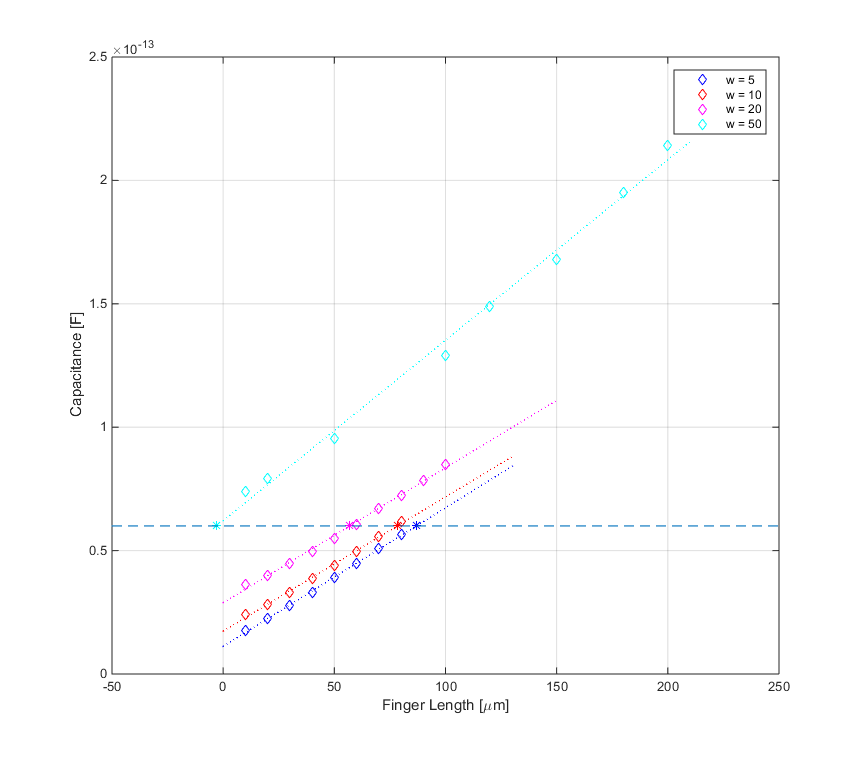
\includegraphics[width = \textwidth]{Figures/Capacitances_g5_50}
	\caption{A plot of the capacitance as a function of finger length for several finger widths. Dashed lines represent linear fits of the data.}
	\label{fig:Capacitances_g5_50}
\end{figure}

\section{The participation ratio}
Using the previous results 